
The TJ-Monopix chip series, as the name suggests, is fabricated by ToweJazz with 180 CMOS imaging process with the goal to find a sensor suitable for future upgrade of experiments.\\
With the same intention and to compare each other \cite{LF-TJ-Monopix}, an other similar sensor has been fabricated bt LFoundrywith 150 CMOSS thecnology: the LF-Monopix is a large-fill factor DMPAS while the TJ-Monopix has a small fill-factor electrode, but both implements a column drain read out with ToT cabability.


\begin{table}
    \begin{center}
    \begin{tabular}{|c | c |c |}
    \hline
    & LF-Monopix & TJ-Monopix\\
    \hline
    \hline

    \hline
    \end{tabular}
    \caption{}
    \label{tab:LF-TJ-Monopix}
    \end{center}
 \end{table}
The modified process employed in TJ-Monopix1 makes use of () $\mu$  thick high resistivity (> 1 k$\Omega$ cm), p-type epitaxial layer grown on a low-ohmic p+ substrate wafer and a low dose implant ().\\

50x50 um2 e l'elettrodo è 3 um

\begin{figure}[h!]
    \centering
    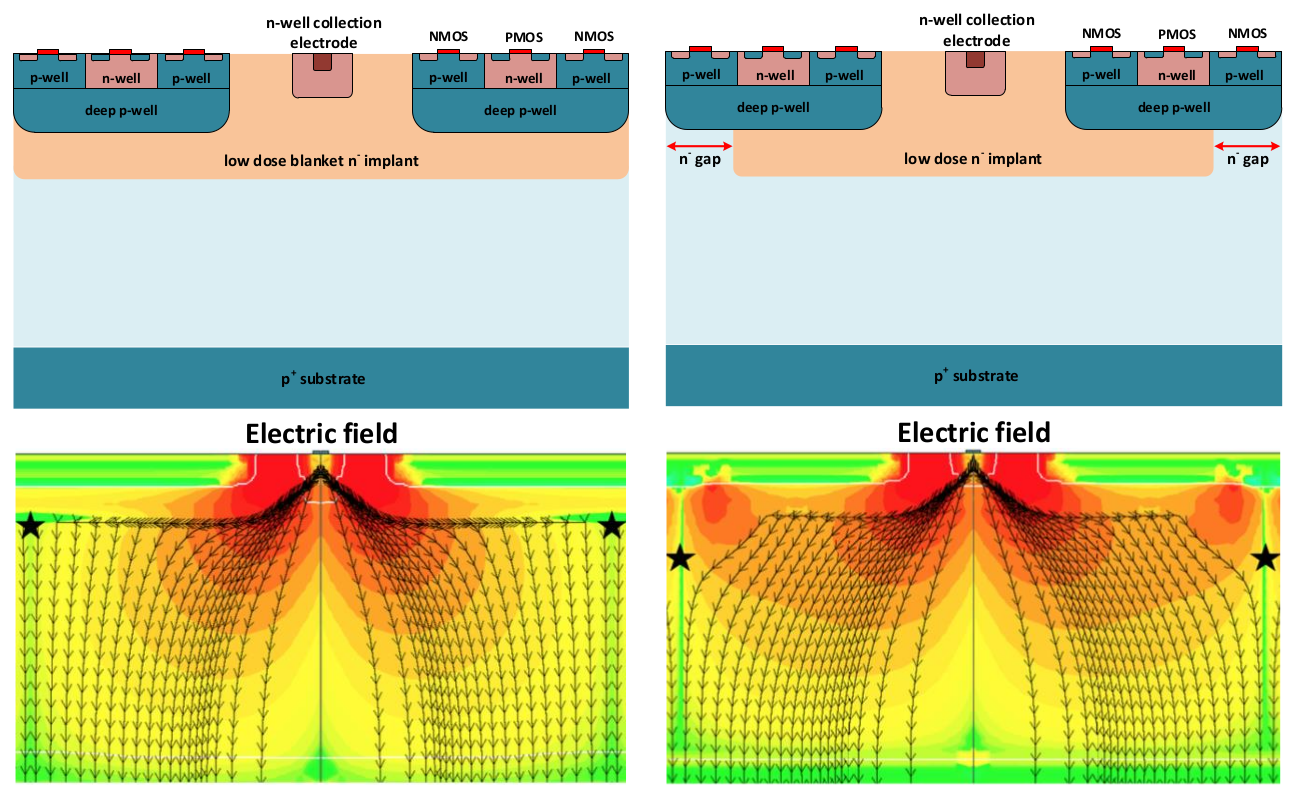
\includegraphics[width=.9\linewidth]{figures/Monopix1/Monopix1_section_scheme.png}
    \caption{(a) The cross-section of a monolithic pixel in the TJ-Monopix 180 nm with modified process; additionaly in (b) a gap in the low dose implant is created to improve the collection of charge due to a bigger lateral component of the electric field}
    \label{fig:Monopix1_section_scheme}
 \end{figure}


\section{FE flavors}
    INput coupling: differenza tra AC (flavor HV) e DC. 4 flavors\\
    \begin{figure}[h!]
        \centering
        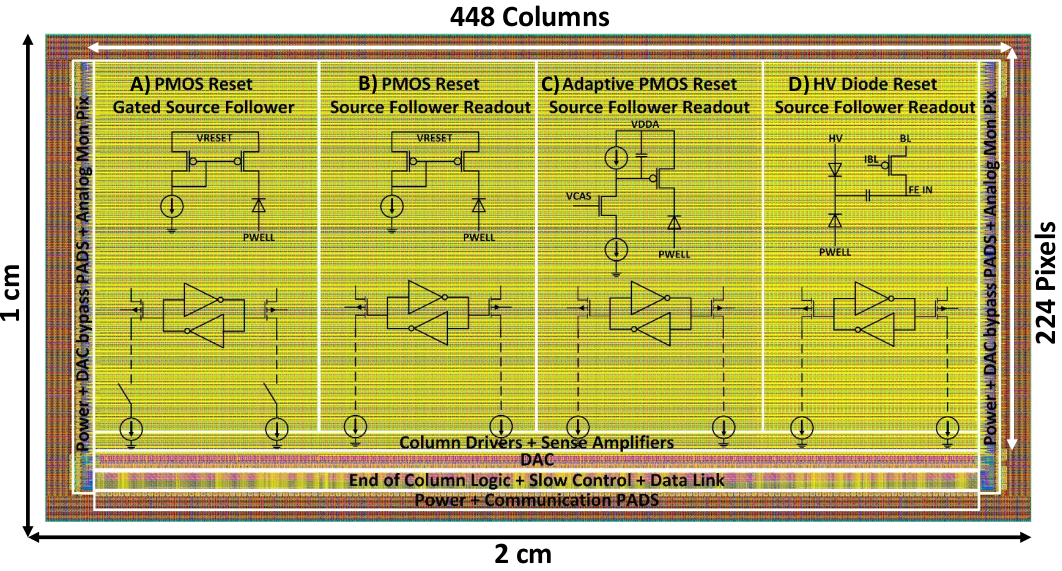
\includegraphics[width=.7\linewidth]{figures/Monopix1/Monopix1_flavors.png}
        \caption{}
        \label{fig:Monopix1_flavors}
    \end{figure}


    \begin{figure}[h!]
        \centering
        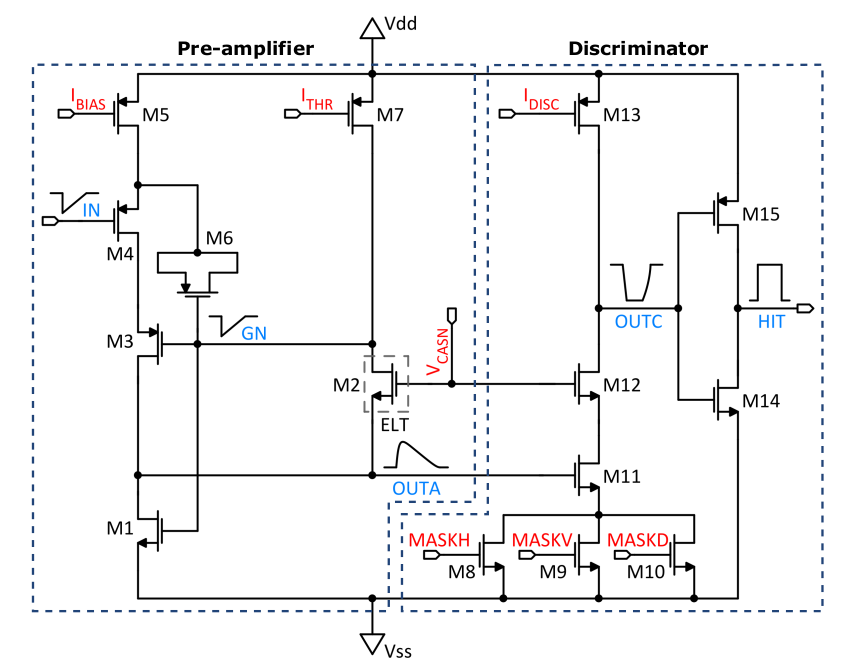
\includegraphics[width=.7\linewidth]{figures/Monopix1/Monopix1_FE_circuit.png}
        \caption{}
        \label{fig:Monopix1_FE_circuit}
    \end{figure}

        R resistenza di reset deve essere abbastanza grande in modo da far si che il
    ritorno allo zero è abbastanza lento (non devi "interferire" con la tot slope
    e non devi più corto del tempo del preamplificatore, sennò hai perdita di segnale).\\
    Baseline reset: all'input solitamente hai un PMOSS o un diodo;  
    Voltage amplifier: perchè? ripeti un attimo il vantaggio. \\
    Source follower per disaccoppiare shaper e LF feedback.\\


\section{Readout logic and sata-packets structure}
    viene da lf monopix\\
    TJ monopix ha un colum drain readout proven by the ATLAS FEI3 front end chip (
    I. Peric et al., The FEI3 readout chip for the ATLAS pixel detector,
    Nucl. Instrum. Meth. A 565 (2006) 178, ed. by J. Grosse-Knetter, H. Krueger, and N. Wermes
    (cit. on pp. 42, 50, 60))\\

    TJ-Monopix is a triggerless. It sends data whenever it gets hits. Only thing we can do is to record timetamp of the external triggers and correlate with the hits. 
    \begin{figure}[h!]
        \centering
        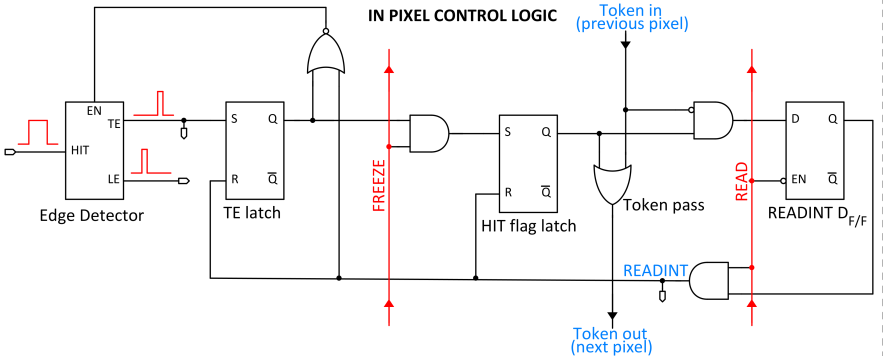
\includegraphics[width=.7\linewidth]{figures/Monopix1/Monopix1_readout_schematics.png}
        \caption{}
        \label{fig:Monopix1_readout_schematics}
    \end{figure}

    \begin{figure}[h!]
        \centering
        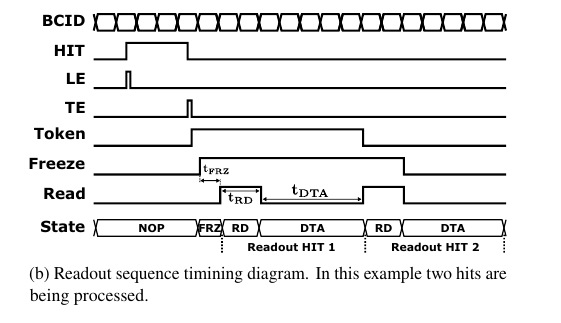
\includegraphics[width=.7\linewidth]{figures/Monopix1/readout_timing.png}
        \caption{}
        \label{fig:readout_timing}
    \end{figure}
    
    \subsection{Dead time measurement}

\section{From TJ-Monopix1 to Obelix}
    Subm. Aug. 2016, mentre monopix 2 sub a aprile 2020\\

    \begin{figure}[h!]
        \centering
        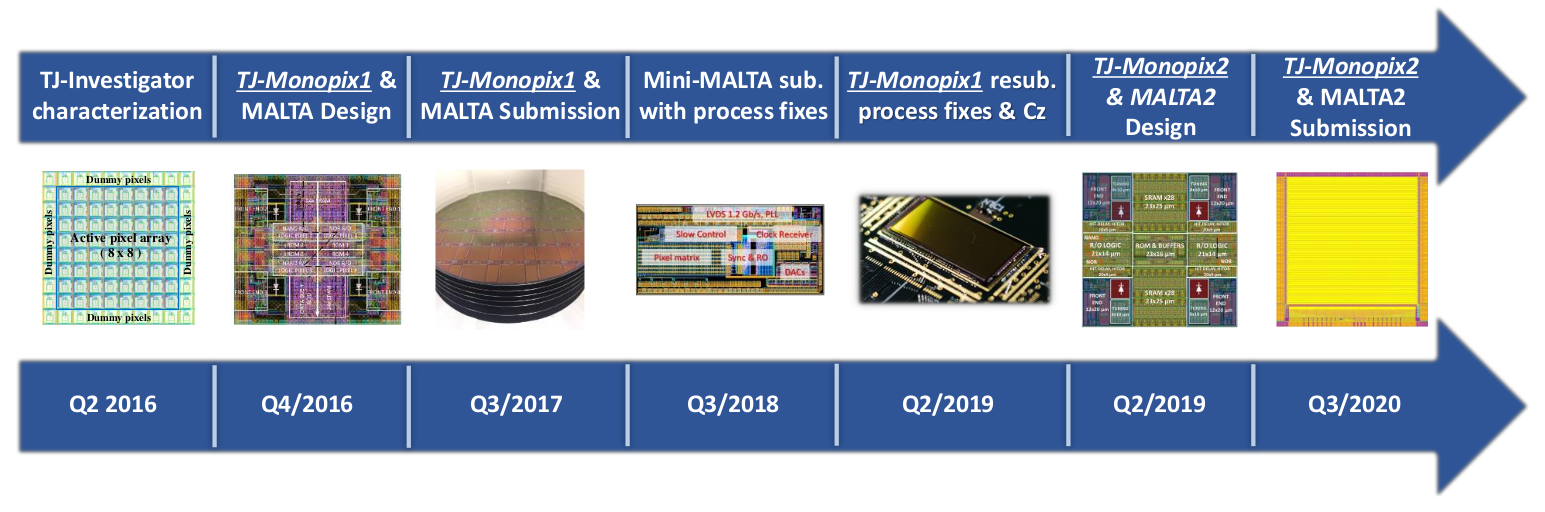
\includegraphics[width=.7\linewidth]{figures/Monopix1/TJ180nm.png}
        \caption{}
        \label{fig:TJ180nm}
    \end{figure}

\section{Applicability to FLASH}
Epitaxial layer thickness: più grande è e più carica viene depositata da una MIP, però devi fare attenzione alla forma della zona svuotata perchè può portare ad un aumento della charge sharing tra pixel vicini. Se il diodo è molto piccolo rischi che l'efficienza di collection è diminutia perchè l'intensità del campo elettrico è più bassa intorno al diodo, e hai più charge sharing.\\